\documentclass[12pt,a4paper]{report}

\usepackage[utf8]{inputenc}
\usepackage[T1]{fontenc}
\usepackage[spanish]{babel}
\usepackage{geometry}
\usepackage{setspace}
\usepackage{titlesec}
\usepackage{hyperref}
\usepackage{graphicx}
\usepackage{float}
\usepackage{longtable}
\usepackage{array}
\usepackage{booktabs}
\usepackage[table]{xcolor}

\geometry{margin=2.5cm}
\onehalfspacing

\begin{document}

%-------------------------
% PORTADA
%-------------------------
\begin{titlepage}
\centering

```
\vspace*{2cm}

{\Huge\bfseries Análisis del Reto\par}

\vspace{2cm}

{\Large Plataforma de Distribución para ISBER Solutions\par}

\vfill

\begin{flushright}
    Autores: Josué Pardo - Alberto Herrera\\
    Carrera: Computación\\
    Universidad: Universidad Técnica Particular de Loja\\
    Fecha: \today
\end{flushright}
```

\end{titlepage}

%-------------------------
% ÍNDICE
%-------------------------
\tableofcontents
\newpage

%-------------------------
% CAPÍTULO 1
%-------------------------
\chapter{Introducción}

\section{Introducción}
ISBER Solutions es una empresa de software ubicada en Loja, Ecuador y planteo el reto de proponer una solución a las dificultades de las empresas de distribución en la ciudad, actualmente enfrentan múltiples contratiempos operativos relacionados con la gestión manual de pedidos, control de inventario, seguimiento de entregas y comunicación entre distribuidores, vendedores y propietarios de tiendas.
El proceso actual depende en gran medida de llamadas telefónicas, mensajes informales y registros manuales para verificar disponibilidad de productos, confirmar pedidos y coordinar entregas. Esta forma de trabajo genera retrasos, errores de comunicación y poca visibilidad del estado real de las operaciones.
Además, la empresa no dispone de una plataforma centralizada que permita controlar de forma eficiente el flujo completo de pedidos desde la creación hasta la entrega final.

\section{Problemática}
La situación actual se caracteriza por una gestión manual de pedidos basada en llamadas y mensajes informales, lo que deriva en pérdida de información, errores en registros y retrasos. Entre los problemas críticos identificados se encuentran:
\begin{itemize}
\item Falta de control de inventario en tiempo real: Los vendedores no conocen el stock disponible, provocando ventas de productos inexistentes.

\item Ausencia de trazabilidad: No existe claridad sobre quién crea, acepta o despacha un pedido, dificultando auditorías y resolución de reclamos.

\item Comunicación ineficiente: Dependencia excesiva de canales informales entre dueños de tiendas, vendedores y repartidores.

\item Falta de evidencia de entrega: Inexistencia de un registro formal o digital que valide la recepción de productos.

\item Escasa capacidad de monitoreo: Ausencia de reportes centralizados para la toma de decisiones estratégicas.
\end{itemize}

\section{Metodología o estrategia de desarrollo}
Para el desarrollo del sistema se adoptó la metodología ágil Scrum, debido a su enfoque iterativo e incremental, que permite entregar funcionalidades funcionales en períodos cortos de tiempo, recibir retroalimentación continua del cliente y adaptarse a cambios en los requisitos del proyecto.

El proyecto se desarrollará durante un período académico de 8 semanas, organizadas en sprints de una semana de duración. Al tratarse de un equipo de dos desarrolladores, ambos participan activamente en las actividades de análisis, diseño, desarrollo, pruebas y despliegue. Los roles de Product Owner y Scrum Master rotan entre los integrantes al inicio de cada sprint para garantizar la participación en todas las responsabilidades definidas por el marco Scrum.

Durante cada sprint se ejecutan las ceremonias principales de Scrum:

Sprint Planning: definición de objetivos y selección de elementos del Product Backlog.
Sprint Review: demostración de los incrementos desarrollados y recopilación de retroalimentación del cliente.
Sprint Retrospective: análisis de fortalezas, problemas y oportunidades de mejora para el siguiente sprint.



%-------------------------
% CAPÍTULO 2
%-------------------------
\chapter{Planificación y análisis}

\section{Análisis}
El análisis realizado en ISBER Solutions permitió identificar diversas deficiencias en los procesos de gestión de pedidos, inventario y entregas. Actualmente, gran parte de las actividades operativas se ejecutan mediante procedimientos manuales o herramientas dispersas, lo que dificulta la coordinación entre distribuidores, vendedores, tiendas y personal de reparto. Esta situación genera retrasos en el procesamiento de pedidos, inconsistencias en los registros de inventario y una limitada capacidad para supervisar el estado de las operaciones en tiempo real.

La ausencia de una plataforma centralizada también afecta la trazabilidad de los procesos. La información se encuentra distribuida entre diferentes actores, dificultando el seguimiento de pedidos, la identificación de responsables ante incidencias y la generación de reportes confiables para la toma de decisiones. Asimismo, la falta de mecanismos automatizados de control incrementa el riesgo de errores humanos, duplicidad de información y pérdida de datos relevantes para la operación.

Desde la perspectiva del negocio, estas limitaciones reducen la eficiencia operativa y restringen la capacidad de crecimiento de la organización. La dependencia de procesos manuales incrementa los tiempos de respuesta, eleva los costos administrativos y afecta la calidad del servicio ofrecido a las tiendas y clientes finales.

Como resultado del análisis, se determinó la necesidad de implementar una plataforma web que centralice la gestión de usuarios, productos, inventario, pedidos y entregas. La solución propuesta permitirá automatizar actividades críticas, mejorar la comunicación entre los diferentes actores, proporcionar trazabilidad completa de las operaciones y disponer de información actualizada para el seguimiento y control del negocio.

La propuesta tecnológica responde directamente a los problemas identificados, incorporando mecanismos de autenticación y control de acceso por roles, gestión de inventario, seguimiento de estados de pedidos, confirmación digital de entregas mediante evidencia fotográfica y herramientas de monitoreo que faciliten la supervisión operativa. De esta manera, se espera mejorar la eficiencia de los procesos, reducir errores operativos y fortalecer la capacidad de gestión de ISBER Solutions.



\section{Requisitos funcionales}
\subsection{RF-01 --- Autenticación}

\begin{longtable}{|p{2cm}|p{2cm}|p{10cm}|}
\hline
\textbf{ID} & \textbf{Prioridad} & \textbf{Requisito} \\ \hline
RF-01.1 & M & El sistema debe permitir a los usuarios registrarse con email, contraseña y un rol preasignado. \\ \hline
RF-01.2 & M & El sistema debe autenticar usuarios mediante email y contraseña. \\ \hline
RF-01.3 & M & El sistema debe permitir solicitar la recuperación de contraseña mediante un enlace de un solo uso enviado al correo registrado. \\ \hline
RF-01.4 & M & El sistema debe permitir establecer una nueva contraseña usando un enlace válido y no expirado. \\ \hline
RF-01.5 & M & El sistema debe invalidar la sesión del usuario al cerrar sesión. \\ \hline
RF-01.6 & M & El enlace de recuperación debe ser de un solo uso y expirar después de 1 hora. \\ \hline
\end{longtable}

\subsection{RF-02 --- Control de Acceso Basado en Roles (RBAC)}

\begin{longtable}{|p{2cm}|p{2cm}|p{10cm}|}
\hline
\textbf{ID} & \textbf{Prioridad} & \textbf{Requisito} \\ \hline
RF-02.1 & M & El sistema debe soportar exactamente cuatro roles: DISTRIBUTOR, VENDOR, STORE\_OWNER, DELIVERY. \\ \hline
RF-02.2 & M & DISTRIBUTOR es el rol de mayor jerarquía; no existe un rol superior dentro del sistema. \\ \hline
RF-02.3 & M & Cada dashboard debe ser accesible únicamente por su rol correspondiente; los accesos no autorizados deben devolver respuesta 403. \\ \hline
RF-02.4 & M & Toda operación que modifique el estado debe revalidar el rol de la sesión en el servidor; nunca se debe confiar en roles enviados por el cliente. \\ \hline
RF-02.5 & M & Todas las consultas deben limitarse al distributorId autenticado; las fugas de datos entre tenants deben ser arquitectónicamente imposibles. \\ \hline
\end{longtable}

\subsection{RF-03 --- Catálogo de Productos (DISTRIBUTOR)}

\begin{longtable}{|p{2cm}|p{2cm}|p{10cm}|}
\hline
\textbf{ID} & \textbf{Prioridad} & \textbf{Requisito} \\ \hline
RF-03.1 & M & El distribuidor debe poder crear productos con: nombre, descripción, precio unitario y stock inicial. \\ \hline
RF-03.2 & M & El distribuidor debe poder actualizar nombre, descripción y precio unitario de un producto. \\ \hline
RF-03.3 & S & El distribuidor debe poder desactivar (soft-delete) un producto; órdenes activas no deben verse afectadas. \\ \hline
RF-03.4 & M & El distribuidor debe poder visualizar el catálogo completo con precios actuales. \\ \hline
RF-03.5 & M & El distribuidor debe poder asignar stock a un vendedor específico creando o actualizando el registro VendorInventory. \\ \hline
\end{longtable}

\subsection{RF-04 --- Gestión de Inventario}

\begin{longtable}{|p{2cm}|p{2cm}|p{10cm}|}
\hline
\textbf{ID} & \textbf{Prioridad} & \textbf{Requisito} \\ \hline
RF-04.1 & M & El distribuidor debe visualizar niveles de stock por producto y vendedor desde el dashboard operativo. \\ \hline
RF-04.2 & M & Un vendedor debe visualizar únicamente su inventario asignado. \\ \hline
RF-04.3 & M & La deducción de inventario debe ejecutarse atómicamente cuando una orden es ACCEPTED, evitando inconsistencias concurrentes. \\ \hline
RF-04.4 & M & Si el inventario es insuficiente durante la aceptación, toda la operación debe revertirse y mostrar un mensaje claro al vendedor. \\ \hline
RF-04.5 & S & El distribuidor debe recibir una alerta visual cuando el stock de un producto caiga por debajo de un umbral configurable. \\ \hline
\end{longtable}

\subsection{RF-05 --- Creación de Órdenes (STORE\_OWNER / VENDOR)}

\begin{longtable}{|p{2cm}|p{2cm}|p{10cm}|}
\hline
\textbf{ID} & \textbf{Prioridad} & \textbf{Requisito} \\ \hline
RF-05.1 & M & Un dueño de tienda debe poder crear órdenes seleccionando productos y cantidades. \\ \hline
RF-05.2 & S & Un vendedor debe poder crear órdenes en nombre de una tienda asignada. \\ \hline
RF-05.3 & M & Al enviar una orden, el sistema debe validar la disponibilidad de productos en el inventario del vendedor objetivo; si algún producto no está disponible, la orden debe rechazarse con errores por ítem. \\ \hline
RF-05.4 & M & El precio de cada ítem debe guardarse al momento de crear la orden y no cambiar si luego cambia el precio del catálogo. \\ \hline
RF-05.5 & M & El dueño de tienda debe visualizar en tiempo real el estado de sus órdenes. \\ \hline
\end{longtable}

\subsection{RF-06 --- Procesamiento de Órdenes (VENDOR)}

\begin{longtable}{|p{2cm}|p{2cm}|p{10cm}|}
\hline
\textbf{ID} & \textbf{Prioridad} & \textbf{Requisito} \\ \hline
RF-06.1 & M & Un vendedor debe visualizar todas las órdenes PENDING asignadas. \\ \hline
RF-06.2 & M & Un vendedor debe poder aceptar o rechazar órdenes pendientes. \\ \hline
RF-06.3 & M & Al aceptar, el inventario debe descontarse atómicamente. \\ \hline
RF-06.4 & M & Al aceptar, la orden pasa a ACCEPTED; al rechazar, a REJECTED. \\ \hline
RF-06.5 & M & El vendedor debe poder marcar órdenes como DISPATCHED cuando salgan de bodega. \\ \hline
RF-06.6 & M & El dashboard del vendedor debe refrescar automáticamente la lista de órdenes pendientes sin recargar manualmente. \\ \hline
\end{longtable}

\subsection{RF-07 --- Confirmación de Entrega (DELIVERY)}

\begin{longtable}{|p{2cm}|p{2cm}|p{10cm}|}
\hline
\textbf{ID} & \textbf{Prioridad} & \textbf{Requisito} \\ \hline
RF-07.1 & M & El personal de entrega debe visualizar órdenes DISPATCHED asignadas a su ruta. \\ \hline
RF-07.2 & M & El personal de entrega debe confirmar las entregas subiendo una foto como evidencia. \\ \hline
RF-07.3 & M & El sistema debe rechazar confirmaciones que no utilicen el flujo oficial de subida de imágenes; URLs externas no son válidas. \\ \hline
RF-07.4 & M & Al confirmar una entrega, la orden cambia a DELIVERED. \\ \hline
RF-07.5 & M & El registro de entrega debe almacenar permanentemente el identificador único de la foto. \\ \hline
\end{longtable}

\section{Requisitos no funcionales}
\subsection{RNF-01 --- Seguridad}

\begin{longtable}{|p{2.5cm}|p{2cm}|p{9.5cm}|}
\hline
\textbf{ID} & \textbf{Prioridad} & \textbf{Requisito} \\ \hline
RNF-01.1 & M & Las contraseñas deben almacenarse mediante hashes criptográficos unidireccionales; nunca texto plano ni cifrado reversible. \\ \hline
RNF-01.2 & M & El acceso a rutas debe validarse en el servidor antes de renderizar contenido. \\ \hline
RNF-01.3 & M & Toda operación que cambie estado debe verificar nuevamente el rol autenticado. \\ \hline
RNF-01.4 & M & Todas las consultas a base de datos deben incluir filtro por distribuidor. \\ \hline
RNF-01.5 & M & Los identificadores de fotos deben validarse para garantizar que provienen del flujo oficial de carga. \\ \hline
RNF-01.6 & M & Los tokens de recuperación de contraseña deben ser de un solo uso. \\ \hline
\end{longtable}

\subsection{RNF-02 --- Rendimiento y Métricas Técnicas}

\begin{longtable}{|p{2.5cm}|p{2cm}|p{9.5cm}|}
\hline
\textbf{ID} & \textbf{Prioridad} & \textbf{Requisito} \\ \hline
RNF-02.1 & M & El tiempo de respuesta de endpoints de listas debe ser $\leq$ 500 ms en el percentil 95 bajo carga normal. \\ \hline
RNF-02.2 & M & La plataforma debe soportar al menos 20 usuarios autenticados concurrentes sin degradación perceptible. \\ \hline
RNF-02.3 & S & Disponibilidad del sistema $\geq$ 99\% durante horario laboral (07:00--20:00 ECT, lunes a sábado). \\ \hline
RNF-02.4 & S & La tasa de error en envío de órdenes no debe superar 1\% bajo condiciones normales. \\ \hline
RNF-02.5 & M & Todas las vistas con relaciones deben usar eager loading; patrones N+1 no son aceptables. \\ \hline
\end{longtable}

\section{Historias de Usuario / Casos de Uso}

Con el propósito de identificar las necesidades de los distintos actores involucrados en el sistema, se definieron historias de usuario basadas en la metodología ágil Scrum. Estas historias describen las funcionalidades que cada rol requiere para cumplir sus actividades dentro del proceso de gestión de pedidos, inventario y entregas.

\begin{longtable}{|p{2cm}|p{12cm}|}
\hline
\textbf{ID} & \textbf{Historia de Usuario} \\ \hline
HU-01 & Iniciar sesión en el sistema mediante correo electrónico y contraseña. \\ \hline
HU-02 & Cerrar sesión de forma segura. \\ \hline
HU-03 & Recuperar la contraseña mediante correo electrónico. \\ \hline
HU-04 & Crear nuevos productos en el catálogo. \\ \hline
HU-05 & Editar la información de productos existentes. \\ \hline
HU-06 & Desactivar productos del catálogo sin afectar pedidos existentes. \\ \hline
HU-07 & Asignar inventario de productos a vendedores. \\ \hline
HU-08 & Consultar el dashboard operativo con información de pedidos e inventario. \\ \hline
HU-09 & Consultar la trazabilidad y auditoría de los pedidos. \\ \hline
HU-10 & Visualizar pedidos pendientes de procesamiento. \\ \hline
HU-11 & Aceptar pedidos y descontar inventario de forma segura. \\ \hline
HU-12 & Rechazar pedidos que no puedan ser atendidos. \\ \hline
HU-13 & Marcar pedidos como despachados. \\ \hline
HU-14 & Realizar pedidos seleccionando productos y cantidades. \\ \hline
HU-15 & Consultar el estado actual de los pedidos realizados. \\ \hline
HU-16 & Recibir notificaciones cuando cambie el estado de un pedido. \\ \hline
HU-17 & Visualizar los pedidos despachados asignados para entrega. \\ \hline
HU-18 & Confirmar la entrega mediante evidencia fotográfica. \\ \hline
HU-19 & Registrar automáticamente los movimientos de inventario para auditoría. \\ \hline
HU-20 & Registrar cambios realizados en el catálogo de productos. \\ \hline
HU-21 & Recibir alertas visuales de inventario bajo. \\ \hline
\end{longtable}

\subsection{Casos de Uso }
Una vez identificadas las historias de usuario y las necesidades funcionales de los diferentes actores del sistema, se procedió a definir los casos de uso que describen de manera detallada la interacción entre los usuarios y la plataforma. Los casos de uso permiten especificar el comportamiento esperado del sistema, estableciendo las acciones que realiza cada actor, las condiciones necesarias para ejecutar un proceso, los posibles escenarios alternativos y los resultados obtenidos al finalizar cada operación.

\begin{longtable}{|p{2cm}|p{12cm}|}
\hline
\textbf{ID} & \textbf{Caso de Uso} \\ \hline
UC-01 & Iniciar Sesión \\ \hline
UC-02 & Cerrar Sesión \\ \hline
UC-03 & Recuperar Contraseña \\ \hline
UC-04 & Gestionar Catálogo de Productos \\ \hline
UC-05 & Asignar Inventario a Vendedor \\ \hline
UC-06 & Visualizar Panel de Operaciones \\ \hline
UC-07 & Consultar Registro de Auditoría \\ \hline
UC-08 & Gestionar Usuarios de la Plataforma \\ \hline
UC-09 & Visualizar Inventario Propio \\ \hline
UC-10 & Visualizar Pedidos Pendientes \\ \hline
UC-11 & Aceptar Pedido \\ \hline
UC-12 & Rechazar Pedido \\ \hline
UC-13 & Marcar Pedido como Despachado \\ \hline
UC-14 & Realizar Pedido \\ \hline
UC-15 & Consultar Estado del Pedido \\ \hline
UC-16 & Visualizar Pedidos Despachados \\ \hline
UC-17 & Confirmar Entrega con Evidencia Fotográfica \\ \hline
\end{longtable}

\subsubsection{UC-01 -- Iniciar Sesión}

\begin{longtable}{|p{4cm}|p{10cm}|}
\hline
\textbf{Atributo} & \textbf{Descripción} \\ \hline
Actores & Distribuidor, Vendedor, Propietario de Tienda, Repartidor. \\ \hline
Precondiciones & El usuario dispone de una cuenta registrada y tiene asignado un rol dentro del sistema. \\ \hline
Flujo Principal &
1. El usuario accede a la pantalla de inicio de sesión.\\
& 2. Ingresa su correo electrónico y contraseña.\\
& 3. El sistema valida las credenciales proporcionadas.\\
& 4. Se crea una sesión autenticada para el usuario.\\
& 5. El sistema redirige al usuario al panel correspondiente a su rol. \\ \hline
Flujo Alternativo A1 & Si la contraseña es incorrecta, el sistema muestra un mensaje genérico de error y no inicia la sesión. \\ \hline
Flujo Alternativo A2 & Si la cuenta no existe, el sistema muestra el mismo mensaje genérico utilizado en el caso anterior para evitar revelar información sobre usuarios registrados. \\ \hline
Postcondiciones & El usuario dispone de una sesión activa y puede acceder a las funcionalidades autorizadas para su rol. \\ \hline
Requisitos Relacionados & RF-01.1, RF-01.2 \\ \hline
\end{longtable}
\subsubsection{UC-03 -- Recuperar Contraseña}

\begin{longtable}{|p{4cm}|p{10cm}|}
\hline
\textbf{Atributo} & \textbf{Descripción} \\ \hline
Actores & Distribuidor, Vendedor, Propietario de Tienda, Repartidor. \\ \hline
Precondiciones & El usuario tiene una dirección de correo electrónico registrada en el sistema. \\ \hline
Flujo Principal &
1. El usuario solicita la recuperación de contraseña ingresando su correo electrónico.\\
& 2. El sistema genera un token único con una vigencia de una hora.\\
& 3. Se envía un enlace de recuperación al correo registrado.\\
& 4. El usuario accede al enlace recibido.\\
& 5. El sistema valida que el token sea válido, no haya sido utilizado y no haya expirado.\\
& 6. El usuario registra una nueva contraseña.\\
& 7. El token queda marcado como utilizado. \\ \hline
Flujo Alternativo A1 & Si el enlace ya fue utilizado, el sistema informa que el enlace no es válido. \\ \hline
Flujo Alternativo A2 & Si el enlace ha expirado, el sistema solicita generar una nueva solicitud de recuperación. \\ \hline
Flujo Alternativo A3 & Si el correo no existe, el sistema muestra una respuesta genérica sin revelar la existencia de la cuenta. \\ \hline
Postcondiciones & La contraseña es actualizada y el usuario puede autenticarse utilizando la nueva credencial. \\ \hline
Requisitos Relacionados & RF-01.3, RF-01.4, RF-01.6 \\ \hline
\end{longtable}
\subsubsection{UC-04 -- Gestionar Catálogo de Productos}

\begin{longtable}{|p{4cm}|p{10cm}|}
\hline
\textbf{Atributo} & \textbf{Descripción} \\ \hline
Actores & Distribuidor. \\ \hline
Precondiciones & El usuario ha iniciado sesión y posee el rol de Distribuidor. \\ \hline
Flujo Principal &
1. El distribuidor accede al módulo de productos.\\
& 2. Registra un nuevo producto indicando nombre, descripción, precio y stock inicial.\\
& 3. El sistema almacena la información asociándola al distribuidor correspondiente.\\
& 4. El producto aparece disponible dentro del catálogo. \\ \hline
Flujo Alternativo A1 & El distribuidor modifica la información de un producto existente. Los cambios se reflejan en el catálogo sin afectar pedidos históricos. \\ \hline
Flujo Alternativo A2 & El distribuidor desactiva un producto para impedir nuevas asignaciones de inventario. \\ \hline
Flujo Alternativo A3 & Si faltan datos obligatorios, el sistema muestra errores de validación y no registra el producto. \\ \hline
Postcondiciones & El catálogo queda actualizado y los productos pueden ser utilizados en los procesos posteriores del sistema. \\ \hline
Requisitos Relacionados & RF-03.1, RF-03.2, RF-03.3, RF-03.4 \\ \hline
\end{longtable}


\subsubsection{UC-05 -- Asignar Inventario a un Vendedor}

\begin{longtable}{|p{4cm}|p{10cm}|}
\hline
\textbf{Atributo} & \textbf{Descripción} \\ \hline
Actores & Distribuidor. \\ \hline
Precondiciones & El producto existe y el usuario seleccionado posee el rol de Vendedor dentro de la misma distribuidora. \\ \hline
Flujo Principal &
1. El distribuidor selecciona un vendedor.\\
& 2. Selecciona el producto a asignar.\\
& 3. Ingresa la cantidad correspondiente.\\
& 4. El sistema crea o actualiza el registro de inventario del vendedor.\\
& 5. La información queda disponible inmediatamente para el vendedor. \\ \hline
Flujo Alternativo A1 & Si la cantidad ingresada es cero, el producto es retirado del inventario del vendedor. \\ \hline
Flujo Alternativo A2 & Si la cantidad es negativa, el sistema rechaza la operación y muestra un mensaje de validación. \\ \hline
Postcondiciones & El inventario asignado al vendedor refleja la cantidad actualizada. \\ \hline
Requisitos Relacionados & RF-03.5, RF-04.1, RF-04.2 \\ \hline
\end{longtable}
\subsubsection{UC-11 -- Aceptar Pedido}

\begin{longtable}{|p{4cm}|p{10cm}|}
\hline
\textbf{Atributo} & \textbf{Descripción} \\ \hline
Actores & Vendedor. \\ \hline
Precondiciones & El pedido existe, se encuentra en estado Pendiente y está asignado al vendedor autenticado. \\ \hline
Flujo Principal &
1. El vendedor visualiza un pedido pendiente.\\
& 2. Selecciona la opción Aceptar Pedido.\\
& 3. El sistema inicia una transacción de base de datos.\\
& 4. Se bloquean temporalmente los registros de inventario involucrados para evitar conflictos concurrentes.\\
& 5. El sistema verifica que exista stock suficiente para todos los productos solicitados.\\
& 6. Se descuenta la cantidad correspondiente del inventario.\\
& 7. El estado del pedido cambia a Aceptado.\\
& 8. El sistema registra el evento en la bitácora de auditoría.\\
& 9. La transacción se confirma y los cambios quedan almacenados. \\ \hline
Flujo Alternativo A1 & Si alguno de los productos no dispone de stock suficiente, la transacción se revierte, el pedido permanece en estado Pendiente y se informa el motivo al vendedor. \\ \hline
Flujo Alternativo A2 & Si dos usuarios intentan aceptar simultáneamente el mismo inventario disponible, solo la primera operación válida se completa; las demás son rechazadas por falta de disponibilidad. \\ \hline
Postcondiciones & El pedido queda registrado como Aceptado, el inventario se actualiza y se genera un registro de auditoría. \\ \hline
Requisitos Relacionados & RF-04.3, RF-04.4, RF-06.2 a RF-06.4, RF-09.1, RF-09.2 \\ \hline
\end{longtable}


\subsubsection{UC-12 -- Rechazar Pedido}

\begin{longtable}{|p{4cm}|p{10cm}|}
\hline
\textbf{Atributo} & \textbf{Descripción} \\ \hline
Actores & Vendedor. \\ \hline
Precondiciones & El pedido existe, se encuentra en estado Pendiente y está asignado al vendedor autenticado. \\ \hline
Flujo Principal &
1. El vendedor consulta un pedido pendiente.\\
& 2. Selecciona la opción Rechazar Pedido.\\
& 3. El sistema solicita confirmación de la acción.\\
& 4. El vendedor confirma el rechazo.\\
& 5. El estado del pedido cambia a Rechazado.\\
& 6. El sistema registra la acción en la bitácora de auditoría. \\ \hline
Flujo Alternativo A1 & Si el vendedor cancela la confirmación, el pedido conserva su estado Pendiente. \\ \hline
Postcondiciones & El pedido queda marcado como Rechazado, sin afectar el inventario disponible. \\ \hline
Requisitos Relacionados & RF-06.2, RF-06.4, RF-09.1 \\ \hline
\end{longtable}


\subsubsection{UC-13 -- Marcar Pedido como Despachado}

\begin{longtable}{|p{4cm}|p{10cm}|}
\hline
\textbf{Atributo} & \textbf{Descripción} \\ \hline
Actores & Vendedor. \\ \hline
Precondiciones & El pedido se encuentra en estado Aceptado y pertenece al vendedor autenticado. \\ \hline
Flujo Principal &
1. El vendedor accede al detalle de un pedido aceptado.\\
& 2. Selecciona la opción Marcar como Despachado.\\
& 3. El sistema solicita confirmación de la acción.\\
& 4. El estado del pedido cambia a Despachado.\\
& 5. Se registra el evento en la bitácora de auditoría.\\
& 6. El pedido pasa a estar disponible para el personal de reparto. \\ \hline
Postcondiciones & El pedido queda en estado Despachado y puede ser gestionado por el personal de entrega. \\ \hline
Requisitos Relacionados & RF-06.5, RF-09.1 \\ \hline
\end{longtable}


\subsubsection{UC-14 -- Realizar Pedido}

\begin{longtable}{|p{4cm}|p{10cm}|}
\hline
\textbf{Atributo} & \textbf{Descripción} \\ \hline
Actores & Propietario de Tienda. \\ \hline
Precondiciones & El usuario ha iniciado sesión como propietario de tienda y existe al menos un vendedor con inventario disponible. \\ \hline
Flujo Principal &
1. El usuario accede al módulo de creación de pedidos.\\
& 2. El sistema muestra los productos disponibles del vendedor correspondiente.\\
& 3. El usuario selecciona los productos y cantidades requeridas.\\
& 4. Envía la solicitud de pedido.\\
& 5. El sistema verifica que todos los productos formen parte del inventario disponible del vendedor.\\
& 6. Se registra el precio vigente de cada producto al momento de la compra.\\
& 7. Se crea el pedido con estado Pendiente.\\
& 8. El sistema confirma el registro exitoso del pedido. \\ \hline
Flujo Alternativo A1 & Si uno o más productos no se encuentran disponibles en el inventario del vendedor, el pedido es rechazado y se muestra el detalle de los errores encontrados. \\ \hline
Flujo Alternativo A2 & Si alguna cantidad ingresada es igual o menor a cero, el sistema solicita corregir la información antes de continuar. \\ \hline
Postcondiciones & El pedido queda registrado en estado Pendiente y disponible para revisión por parte del vendedor. \\ \hline
Requisitos Relacionados & RF-05.1, RF-05.3, RF-05.4 \\ \hline
\end{longtable}


\subsubsection{UC-17 -- Confirmar Entrega con Evidencia Fotográfica}

\begin{longtable}{|p{4cm}|p{10cm}|}
\hline
\textbf{Atributo} & \textbf{Descripción} \\ \hline
Actores & Repartidor. \\ \hline
Precondiciones & El pedido se encuentra en estado Despachado y está asignado al repartidor correspondiente. \\ \hline
Flujo Principal &
1. El repartidor accede al detalle del pedido despachado.\\
& 2. Adjunta una fotografía como evidencia de la entrega.\\
& 3. La imagen es cargada al servicio de almacenamiento configurado para la plataforma.\\
& 4. El sistema recibe el identificador único de la fotografía.\\
& 5. El repartidor envía la confirmación de entrega.\\
& 6. El sistema valida que la evidencia fotográfica sea válida y haya sido generada mediante la plataforma.\\
& 7. Se registra la evidencia en la base de datos.\\
& 8. El estado del pedido cambia a Entregado.\\
& 9. El sistema registra la acción en la bitácora de auditoría. \\ \hline
Flujo Alternativo A1 & Si la evidencia fotográfica no supera las validaciones establecidas, la confirmación es rechazada y el pedido permanece en estado Despachado. \\ \hline
Flujo Alternativo A2 & Si no se adjunta una fotografía, el sistema impide completar el proceso de confirmación. \\ \hline
Postcondiciones & El pedido queda registrado como Entregado, junto con la evidencia fotográfica correspondiente y el registro de auditoría asociado. \\ \hline
Requisitos Relacionados & RF-07.1 a RF-07.5, RF-09.1 \\ \hline
\end{longtable}

\section{Sprint}
El desarrollo del sistema se planificó mediante la metodología Scrum, organizando el trabajo en 8 sprints de una semana de duración cada uno. Cada sprint tiene como objetivo entregar un incremento funcional del producto, permitiendo validar avances de manera continua, identificar riesgos tempranamente y obtener retroalimentación para la planificación de las siguientes iteraciones.

Sprint 1 – Configuración del Entorno y Base del Proyecto.
Sprint 2 – Autenticación y Control de Acceso
Sprint 3 – Gestión de Catálogo
Sprint 4 – Gestión de Inventario
Sprint 5 – Gestión de Pedidos
Sprint 6 – Entrega y Auditoría
Sprint 7 – Dashboard y Funcionalidades Complementarias
Sprint 8 – Pruebas Integrales, Corrección de Incidencias y Despliegue	


\section{Diagramas: Clases y BD (diseño lógico) – Preguntas y respuesta al diagrama }

    \begin{figure}[H]
    \centering
    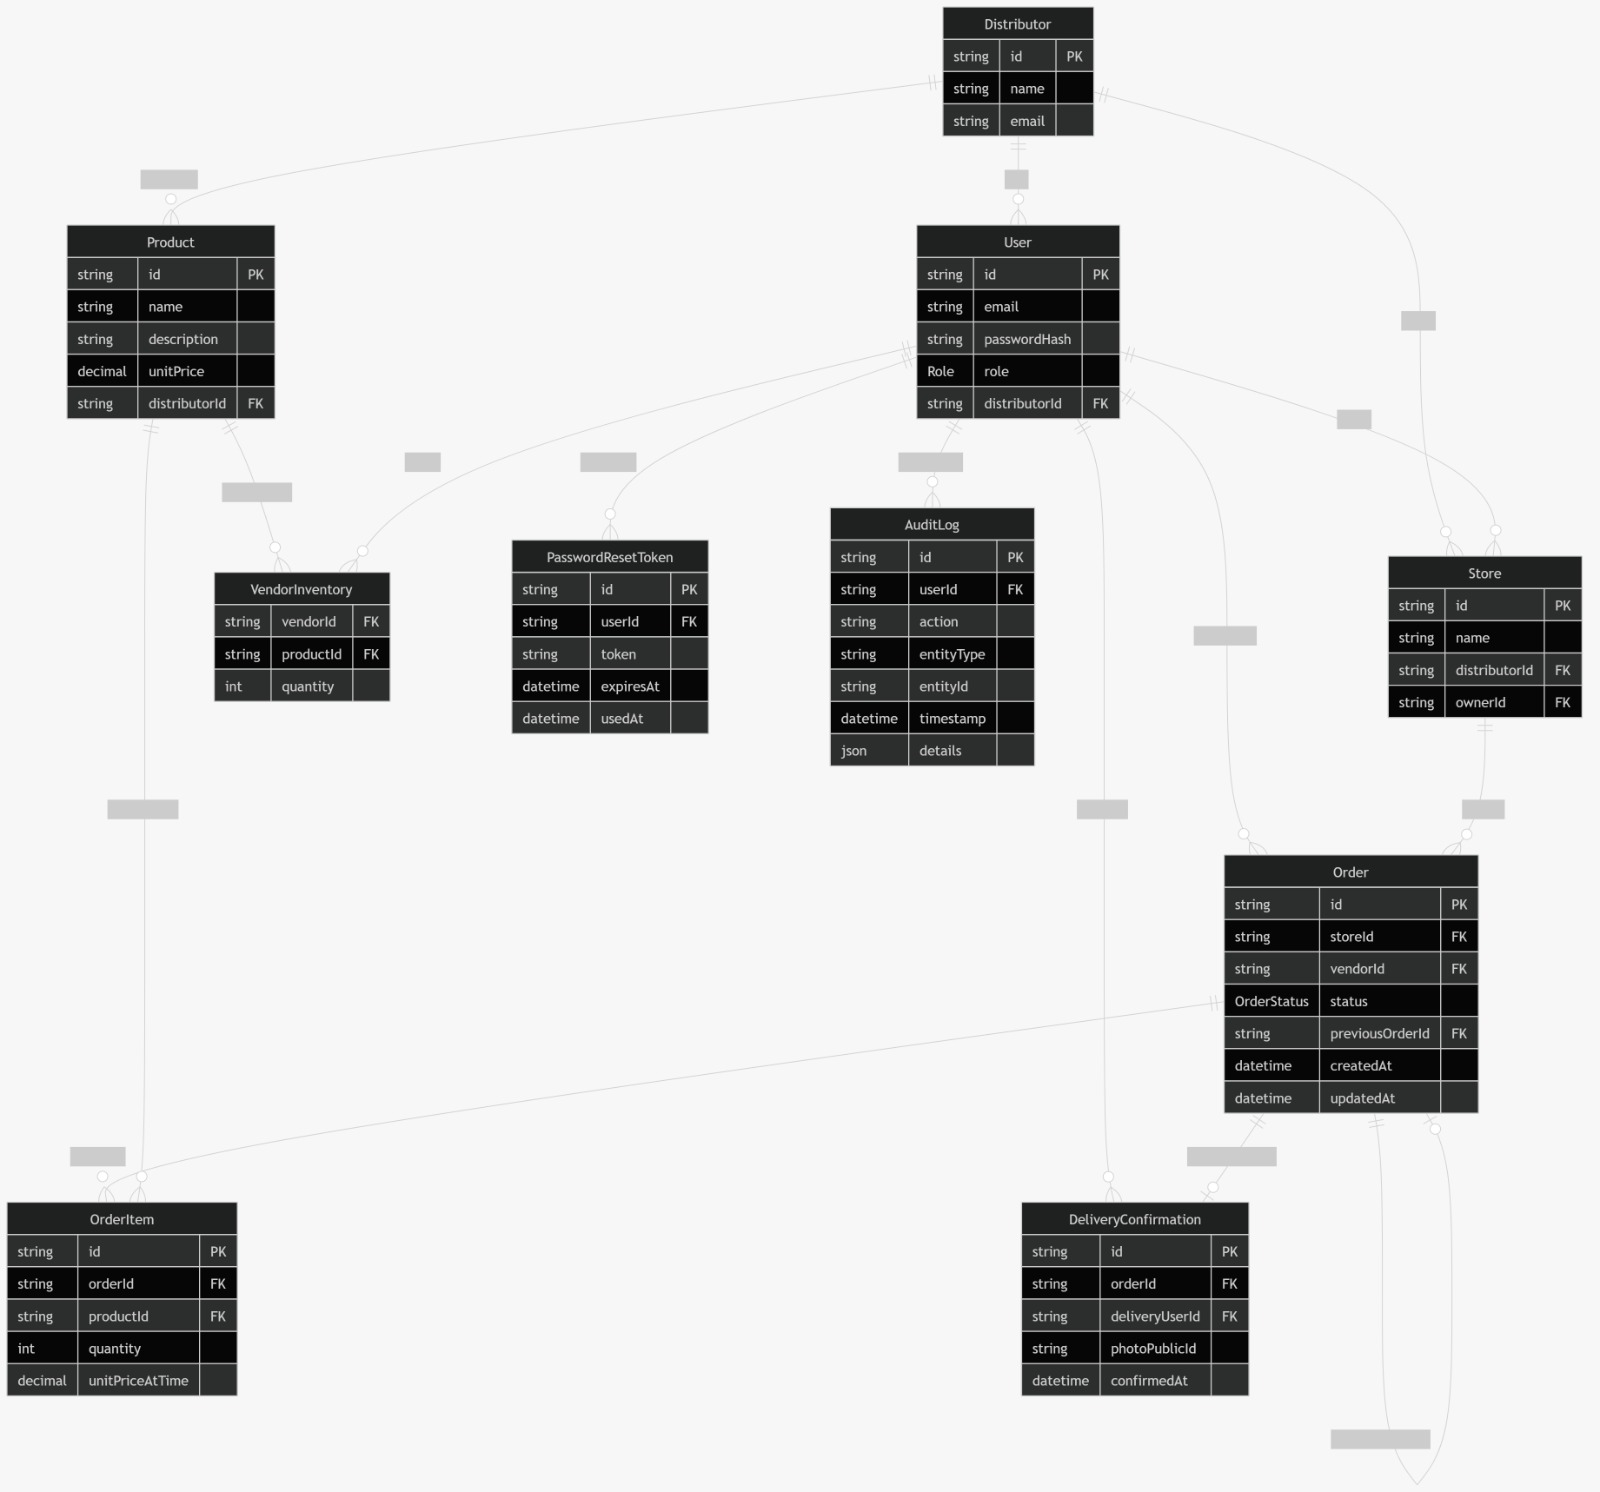
\includegraphics[width=0.5\linewidth]{diagrama_de_clases.jpeg}
    \caption{Diagrama de Clases}
    \label{fig:clases}
\end{figure}
   

\subsection{Preguntas y respuestas del diagrama}
\begin{enumerate}
\item Pregunta 1. ¿Cómo garantiza el diseño del esquema el aislamiento de datos (multi-tenancy) para que diferentes distribuidoras no puedan acceder a la información de las demás?

La entidad Distributor actúa como eje central del modelo y se relaciona mediante la clave foránea distributorId con entidades como User, Store y Product. Gracias a esta estructura, todas las consultas pueden filtrarse por distribuidora, garantizando que cada organización únicamente acceda a sus propios usuarios, tiendas, productos y operaciones. Este enfoque permite cumplir con los requisitos de seguridad y confidencialidad, evitando fugas de información entre distribuidoras.

\item Pregunta 2. ¿Cómo puede determinarse qué distribuidora tiene el mayor volumen de ventas en un período determinado?

La consulta requiere relacionar las entidades Distributor, Store, Order y OrderItem. A través de la tienda se identifica la distribuidora propietaria, mientras que los ítems del pedido almacenan la cantidad vendida y el precio registrado en unitPriceAtTime. Esto permite calcular ingresos históricos reales por distribuidora, incluso cuando los precios actuales de los productos hayan cambiado posteriormente.

\item Pregunta 3. ¿De qué manera el esquema resuelve el problema de la pérdida de integridad en los precios históricos cuando el distribuidor actualiza el costo de un producto en el catálogo?

La solución se encuentra en la separación entre las entidades Product y OrderItem. Mientras Product almacena el precio actual del producto, OrderItem conserva el valor del campo unitPriceAtTime, registrando el precio exacto existente al momento de crear el pedido. De esta forma, los reportes históricos, facturación y análisis financieros permanecen consistentes aunque los precios del catálogo sean modificados posteriormente.

\item Pregunta 4. ¿Qué estructura permite al sistema controlar que un vendedor solo venda los productos y cantidades que tiene asignados?:

La entidad VendorInventory vincula a un usuario con rol vendedor (User) con un producto (Product) y una cantidad específica disponible. Esta tabla funciona como un inventario individual por vendedor, independiente del stock general de la distribuidora. Antes de aceptar una orden, el sistema puede verificar la existencia y disponibilidad en esta asignación, garantizando que el vendedor únicamente comercialice productos autorizados.

\item Pregunta 5. ¿Cómo permite el diagrama reconstruir la línea de tiempo completa de una orden que fue rechazada, modificada y procesada posteriormente?

Aunque la entidad Order conserva únicamente el estado actual del pedido, la trazabilidad histórica se obtiene mediante AuditLog. Esta entidad registra el usuario responsable (userId), la acción ejecutada (action), la entidad afectada (entityType), el identificador correspondiente (entityId) y detalles adicionales en formato JSON. Gracias a estos registros es posible reconstruir cronológicamente todos los eventos ocurridos sobre una orden, identificar responsables y realizar auditorías completas del proceso.



\end{enumerate}

\section{Diagrama de Componentes}

\begin{figure}[H]
    \centering
    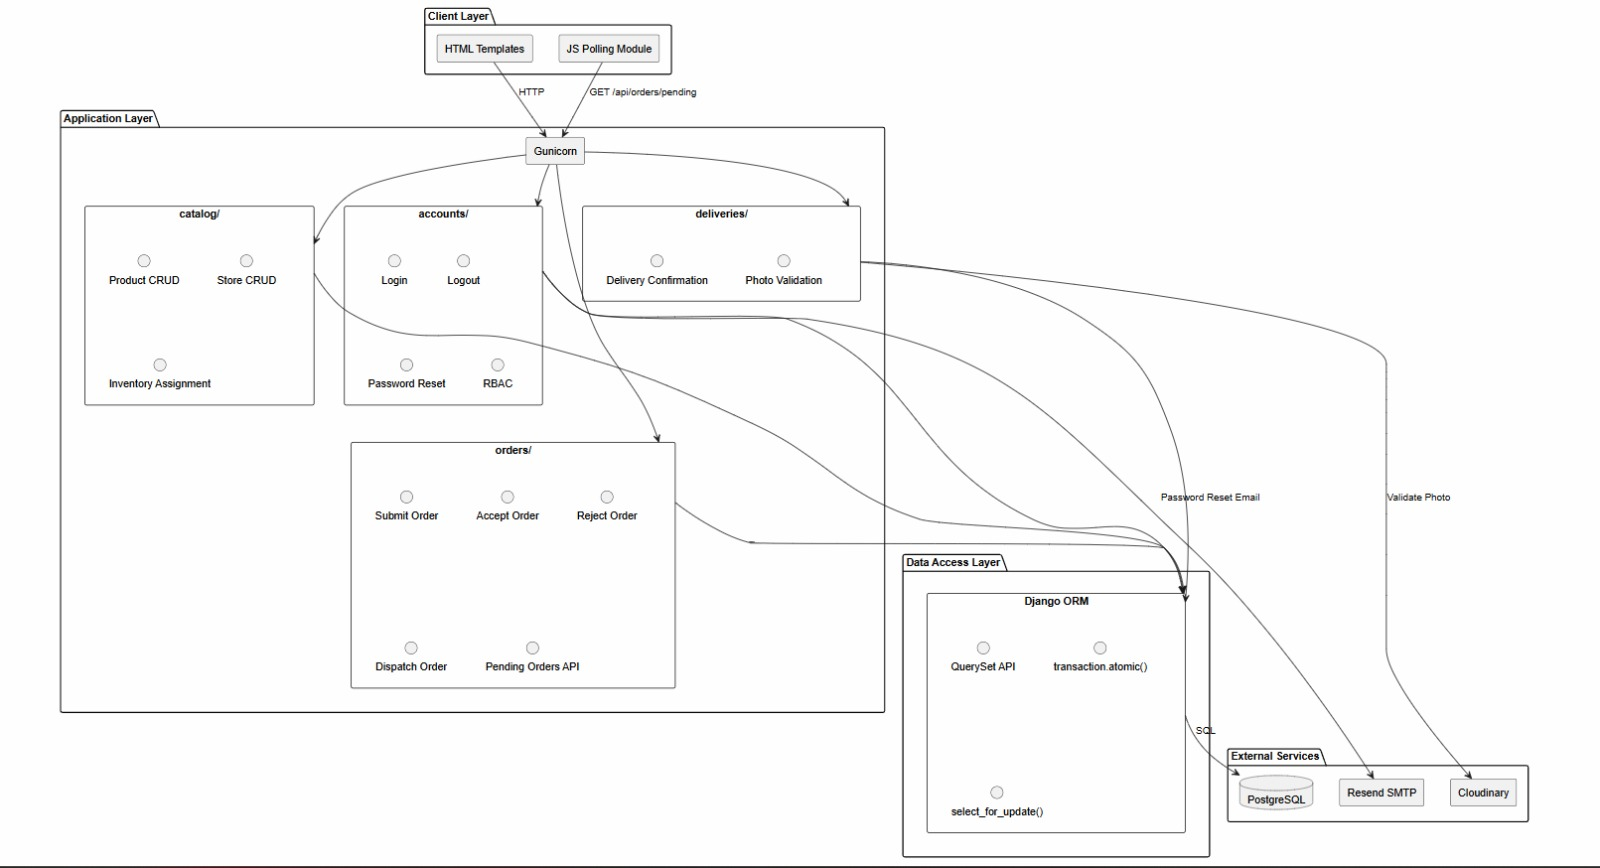
\includegraphics[width=\textwidth]{diagrama_componentes.jpeg}
    \caption{Diagrama de Componentes}
    \label{fig:componentes}
\end{figure}
La arquitectura del sistema se basa en un modelo de capas que promueve la separación de responsabilidades y facilita el mantenimiento, escalabilidad y seguridad de la aplicación. Las solicitudes de los usuarios se originan en la capa cliente, donde se presentan las interfaces web y se ejecutan mecanismos de actualización periódica mediante JavaScript. Estas solicitudes son procesadas por la capa de aplicación implementada con Django, la cual gestiona la autenticación, autorización basada en roles, validaciones de negocio y el flujo de las operaciones principales del sistema.

La capa de acceso a datos utiliza el ORM de Django para abstraer la comunicación con la base de datos PostgreSQL, garantizando la integridad transaccional, el aislamiento de datos entre distribuidoras y la optimización de consultas. Finalmente, la arquitectura integra servicios externos especializados para funciones complementarias, como el almacenamiento de evidencias fotográficas mediante Cloudinary y el envío de correos electrónicos a través de Resend. Esta organización permite desacoplar los componentes del sistema, mejorar la mantenibilidad del código y asegurar un flujo de comunicación controlado entre cada una de las capas.


\section{Arquitectura lógica y física (Propuesta)}

La arquitectura propuesta para el sistema ha sido diseñada con el objetivo de garantizar una adecuada separación de responsabilidades, facilitar el mantenimiento de la aplicación y permitir su crecimiento futuro sin afectar significativamente los componentes existentes. Para ello, se adopta una arquitectura multicapa basada en el patrón MVT (Model-View-Template) de Django, donde cada capa cumple una función específica dentro del procesamiento de las solicitudes y la gestión de la información.

Desde la perspectiva lógica, la solución organiza sus componentes en capas de presentación, aplicación, servicios transversales, dominio y acceso a datos. Esta estructura permite desacoplar la interfaz de usuario de la lógica de negocio y del almacenamiento de información, facilitando la implementación de mecanismos de seguridad, control de acceso basado en roles, auditoría de acciones y aislamiento de datos entre distribuidoras. Asimismo, favorece la reutilización de componentes y la mantenibilidad del sistema durante futuras fases de evolución.

Desde la perspectiva física, la arquitectura se apoya en una infraestructura basada en servicios en la nube. La aplicación se ejecuta sobre Railway utilizando Django y Gunicorn como plataforma de ejecución, mientras que PostgreSQL se emplea como sistema gestor de base de datos. Adicionalmente, se integran servicios externos especializados para el almacenamiento de evidencias fotográficas y el envío de correos electrónicos. Esta distribución permite aprovechar servicios administrados, reducir la complejidad operativa y mejorar la gestión operativa de la infraestructura mediante el uso de servicios administrados en la nube.-

La combinación de ambas arquitecturas proporciona una solución alineada con los requisitos funcionales y no funcionales del proyecto, garantizando seguridad, escalabilidad, mantenibilidad e integridad de la información, al tiempo que permite una comunicación eficiente entre usuarios, aplicación, base de datos y servicios externos.


\section{Prototipo de pantallas no funcional}
El diseño contempla dashboards específicos por rol:
Vista de Inventario: Niveles de stock visuales con alertas cuando el producto está bajo el umbral.
Dashboard de Pedidos: Lista con refresco automático cada 30 segundos (vía polling) para monitorear órdenes pendientes.
Interfaz de Entrega: Módulo de carga de archivos para la evidencia fotográfica del personal de reparto.
\subsection{Pantalla principal(Dashboard General del Distribuidor)}
La Figura 2.3 presenta el panel principal de operaciones del distribuidor dentro de la plataforma ISBER Solutions. Esta interfaz ha sido diseñada para proporcionar una visión consolidada y en tiempo real de los principales indicadores operativos relacionados con la gestión de pedidos, inventario y recursos comerciales.
\begin{figure}[H]
    \centering
    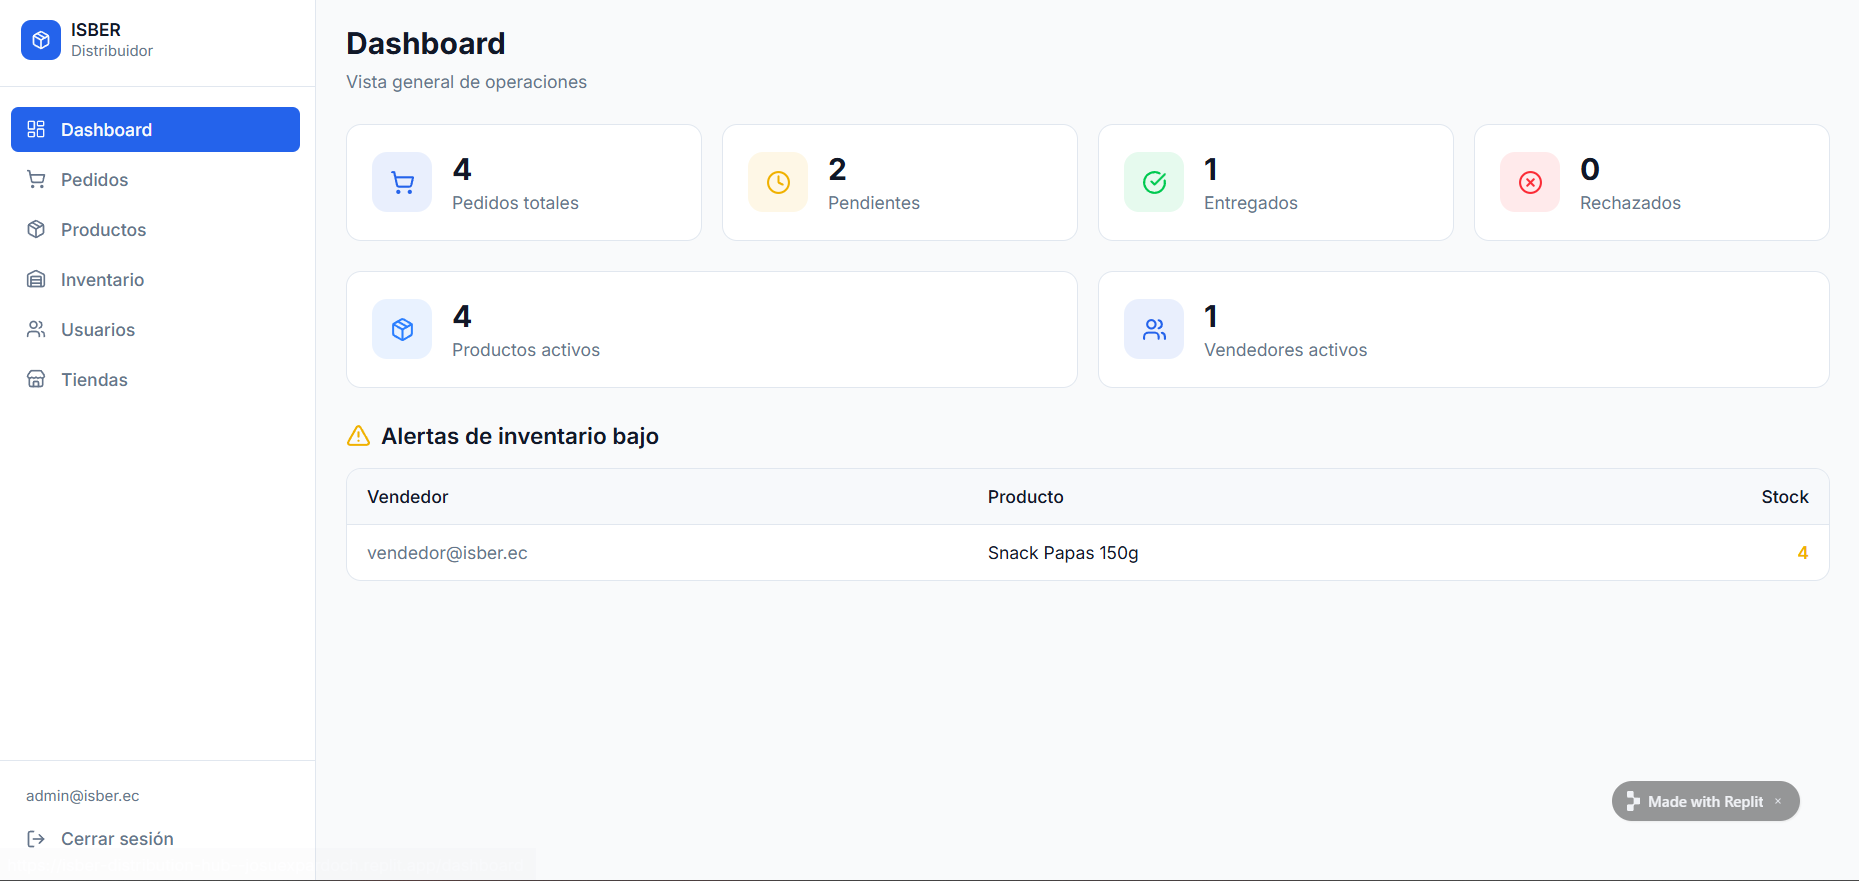
\includegraphics[width=0.5\linewidth]{image.png}
    \caption{Enter Caption}
    \label{fig:placeholder}
\end{figure}

\subsection{Pantalla de gestión (Gestión y Seguimiento de Pedidos de la Tienda)}
La Figura 2.4 presenta la interfaz de gestión de pedidos disponible para los propietarios de tiendas dentro de la plataforma ISBER Solutions. Este módulo permite a los usuarios consultar el historial de pedidos realizados, monitorear su estado en tiempo real y generar nuevas solicitudes de abastecimiento de manera centralizada.
\begin{figure}[H]
    \centering
    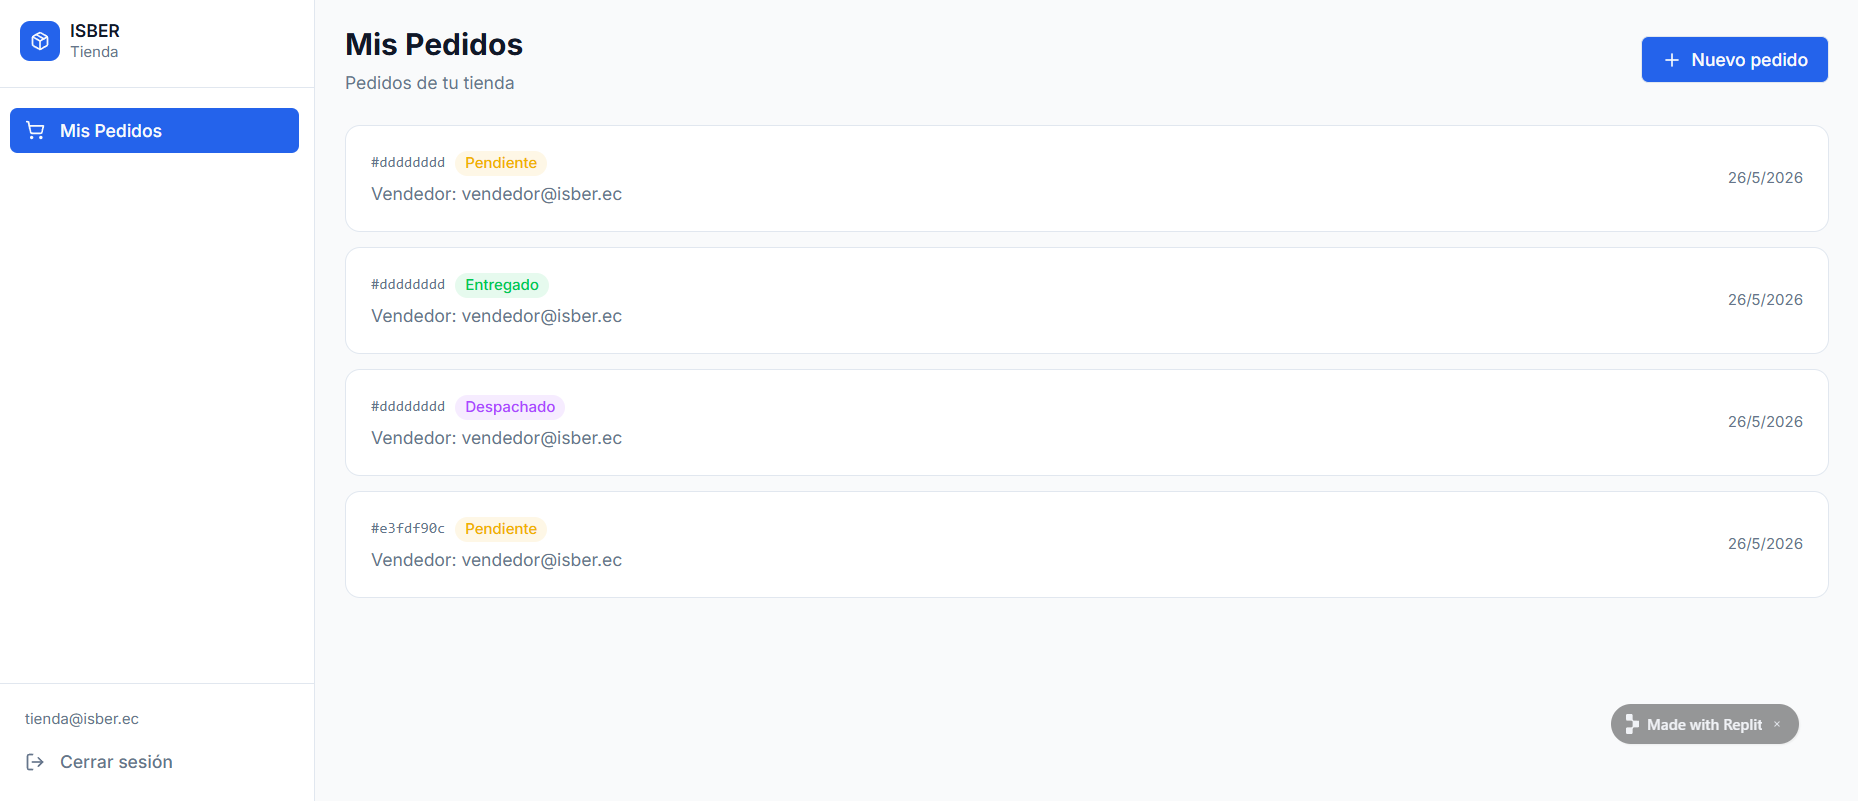
\includegraphics[width=0.5\linewidth]{image1.png}
    \caption{Enter Caption}
    \label{fig:placeholder}
\end{figure}

\end{document}
